\documentclass[12pt, a4paper]{report}

% --- Pakiety i kodowanie ---
\usepackage[utf8]{inputenc}
\usepackage[T1]{fontenc}
\usepackage[polish]{babel}  % Język polski
\usepackage{graphicx}       % Obsługa obrazków
\usepackage{geometry}       % Marginesy
\usepackage{csquotes}       % Cudzysłowy
\usepackage{float}          % Pozycjonowanie tabel/obrazków
\usepackage{hyperref}       % Linki w dokumencie
\usepackage{fancyhdr}       % Własne nagłówki i stopki
\usepackage{titlesec}       % Formatowanie tytułów

% --- Bibliografia ---
\usepackage[backend=biber, style=numeric]{biblatex}
\addbibresource{references.bib}

% --- Ustawienia marginesów ---
\geometry{
 left=25mm,
 right=25mm,
 top=25mm,
 bottom=25mm
}

% --- Dane autora ---
\newcommand{\autorImieNazwisko}{Mikołaj Zdybiewski} % <-- Imie i nazwisko autor
\newcommand{\tytulPracy}{Wprowadzenie do Sztucznej Inteligencji}

% --- KONFIGURACJA NAGŁÓWKÓW ---
\pagestyle{fancy}
\fancyhf{} 

% Ustawienia dla standardowych stron
\fancyhead[L]{\nouppercase{\leftmark}} % Lewy górny: Tytuł rozdziału
\fancyhead[R]{\autorImieNazwisko}      % Prawy górny: Autor (Mikołaj Zdybiewski)
\fancyfoot[C]{\thepage}                % Dół środek: Numer strony

% Usunięcie słowa "Rozdział X" z nagłówka
\renewcommand{\chaptermark}[1]{\markboth{\thechapter.\ #1}{}}

% --- WYMUSZENIE NAGŁÓWKA NA STRONACH STARTOWYCH ROZDZIAŁÓW ---
\fancypagestyle{plain}{
    \fancyhf{} 
    \fancyhead[L]{\nouppercase{\leftmark}} 
    \fancyhead[R]{\autorImieNazwisko}      
    \fancyfoot[C]{\thepage}
}

% --- POCZĄTEK DOKUMENTU ---
\begin{document}

% --- Strona tytułowa ---
\begin{titlepage}
    \centering
    \vspace*{1cm}
    \Huge \textbf{\tytulPracy}
    \vspace{1.5cm}
    
    \Large \textbf{Raport zaliczeniowy}
    \vspace{1.5cm}
    
    \textbf{Autor:} \\ \autorImieNazwisko
    \vspace{4cm}
    
    \textbf{Data:} \\ 5 grudnia 2025
    \vfill
    
    \Large Politechnika Wrocławska\\Wydział Informatyki i Telekomunikacji
\end{titlepage}

% --- Streszczenie ---
\begin{abstract}
    \noindent Dokument stanowi wprowadzenie do tematyki sztucznej inteligencji, omawiając jej historię, rodzaje oraz zastosowania. Jest to projekt zaliczeniowy prezentujący umiejętności składu tekstu w systemie \LaTeX, w tym obsługę bibliografii, tabel i grafik, z zachowaniem spójnych nagłówków i struktury dokumentu.
\end{abstract}

% --- Spis treści ---
\tableofcontents
\newpage

% --- Dołączanie rozdziałów ---
\chapter{Wstęp do problematyki AI}

Sztuczna inteligencja (AI) to dziedzina informatyki zajmująca się tworzeniem systemów zdolnych do wykonywania zadań, które normalnie wymagałyby ludzkiej inteligencji. Zadania te obejmują m.in. rozpoznawanie obrazów, przetwarzanie języka naturalnego, podejmowanie decyzji w warunkach niepewności oraz tłumaczenie między językami. Jak zauważają Russell i Norvig w swojej fundamentalnej pracy, jest to nauka o agentach, którzy odbierają bodźce z otoczenia za pomocą sensorów i podejmują działania za pomocą efektorów, dążąc do maksymalizacji określonej miary użyteczności \cite{russell2020}.

W ostatnich dekadach obserwujemy gwałtowny rozwój tej dziedziny, co wynika z trzech głównych czynników:
\begin{enumerate}
    \item \textbf{Dostępność danych} -- żyjemy w erze Big Data, gdzie ilość generowanych informacji cyfrowych rośnie wykładniczo, dostarczając "paliwa" dla algorytmów uczących się.
    \item \textbf{Moc obliczeniowa} -- rozwój kart graficznych (GPU) oraz dedykowanych układów tensorowych (TPU) umożliwił trenowanie ogromnych sieci neuronowych w rozsądnym czasie.
    \item \textbf{Nowe algorytmy} -- udoskonalenie metod takich jak wsteczna propagacja błędu czy architektura Transformer.
\end{enumerate}

Współczesne systemy AI opierają się głównie na uczeniu maszynowym (\textit{Machine Learning}) oraz jego poddziedzinie -- uczeniu głębokim (\textit{Deep Learning}). W przeciwieństwie do klasycznego programowania, gdzie człowiek definiuje reguły, w uczeniu maszynowym system samodzielnie ekstrahuje wzorce z dostarczonych danych treningowych. Celem tego raportu jest przedstawienie kluczowych aspektów tej technologii, jej historii oraz wpływu na współczesny świat.
\chapter{Historia i rodzaje AI}

Rozwój sztucznej inteligencji nie był procesem liniowym; dziedzina ta przeżywała okresy wielkiego optymizmu, przeplatane tzw. "zimami AI", kiedy to fundusze na badania były drastycznie obcinane z powodu braku spektakularnych sukcesów. Początki teoretyczne sięgają prac Alana Turinga, który w 1950 roku w czasopiśmie "Mind" zadał kluczowe pytanie "Czy maszyny mogą myśleć?" i zaproponował test (znany dziś jako Test Turinga) mający na celu weryfikację inteligencji maszynowej \cite{turing1950}.

\section{Kamienie milowe rozwoju}
Analizując historię sztucznej inteligencji, można wyróżnić momenty przełomowe, które zmieniały postrzeganie możliwości komputerów. Poniżej przedstawiono wybrane wydarzenia (lista numerowana):

\begin{enumerate}
    \item \textbf{1950} -- Publikacja pracy Alana Turinga, która położyła podwaliny pod filozofię sztucznej inteligencji.
    \item \textbf{1956} -- Konferencja w Dartmouth, zorganizowana przez Johna McCarthy'ego. To właśnie tam oficjalnie ukuto termin "Artificial Intelligence" i wyznaczono kierunki badań na kolejne dekady.
    \item \textbf{1997} -- System Deep Blue firmy IBM wygrywa mecz szachowy z ówczesnym mistrzem świata, Garrim Kasparowem. Był to pierwszy dowód na to, że maszyna może przewyższyć człowieka w grze strategicznej wymagającej planowania.
    \item \textbf{2012} -- Przełom w rozpoznawaniu obrazów dzięki sieci AlexNet, co zapoczątkowało rewolucję Głębokiego Uczenia (\textit{Deep Learning}).
    \item \textbf{2022} -- Publiczne udostępnienie modelu ChatGPT przez OpenAI, co spopularyzowało generatywną sztuczną inteligencję wśród setek milionów użytkowników na całym świecie.
\end{enumerate}

\section{Klasyfikacja systemów AI}
W literaturze przedmiotu oraz w dyskursie publicznym systemy AI dzieli się zazwyczaj ze względu na ich zakres kompetencji i poziom zaawansowania (lista nienumerowana):

\begin{itemize}
    \item \textbf{ANI (Artificial Narrow Intelligence)} -- sztuczna inteligencja wąska. Są to systemy wyspecjalizowane w wykonywaniu jednego, konkretnego zadania, często lepiej niż człowiek. Przykłady to algorytmy grające w szachy, systemy rekomendacji Netflixa czy filtry antyspamowe. Obecnie wszystkie istniejące systemy AI należą do tej kategorii.
    
    \item \textbf{AGI (Artificial General Intelligence)} -- ogólna sztuczna inteligencja. Jest to hipotetyczny system, który posiadałby zdolność uczenia się i rozumienia świata na poziomie zbliżonym do człowieka. AGI potrafiłaby przenieść wiedzę z jednej dziedziny do innej i rozwiązywać problemy, z którymi wcześniej się nie zetknęła.
    
    \item \textbf{ASI (Artificial Super Intelligence)} -- superinteligencja. Termin ten określa intelekt znacznie przewyższający możliwości kognitywne najmądrzejszych ludzi we wszystkich dziedzinach, włączając w to kreatywność naukową, mądrość ogólną i kompetencje społeczne.
\end{itemize}
\chapter{Zastosowania praktyczne}

Sztuczna inteligencja przestała być jedynie domeną badań akademickich i stała się integralną częścią globalnej gospodarki. Znajduje zastosowanie w medycynie (diagnostyka obrazowa), transporcie (pojazdy autonomiczne), finansach (wykrywanie oszustw) oraz przemyśle rozrywkowym. Największe emocje w ostatnich latach budzą jednak Duże Modele Językowe (LLM).

\section{Analiza porównawcza modeli językowych}
Współczesne modele językowe różnią się architekturą, zbiorem danych użytym do treningu oraz liczbą parametrów, która często koreluje z ich możliwościami. Zestawienie popularnych rozwiązań przedstawia Tabela \ref{tab:modele}. Warto zauważyć, że nowsze modele, takie jak GPT-4, wykazują zdolności multimodalne, co oznacza, że potrafią przetwarzać nie tylko tekst, ale i obrazy.

\begin{table}[H]
    \centering
    \caption{Porównanie popularnych modeli językowych}
    \label{tab:modele}
    \begin{tabular}{|l|c|l|l|}
        \hline
        \textbf{Model} & \textbf{Rok} & \textbf{Firma} & \textbf{Główne zastosowanie} \\
        \hline
        BERT & 2018 & Google & Rozumienie kontekstu \\
        \hline
        GPT-4 & 2023 & OpenAI & Generowanie tekstu i kodu \\
        \hline
        Llama 2 & 2023 & Meta & Open Source, badania \\
        \hline
    \end{tabular}
\end{table}

\section{Wizualizacja procesów uczenia}
Podstawą działania większości nowoczesnych systemów AI są sztuczne sieci neuronowe. Są one luźno inspirowane budową biologicznego mózgu. Składają się z warstw neuronów: warstwy wejściowej, wielu warstw ukrytych oraz warstwy wyjściowej. Informacja przepływa przez sieć, a wagi połączeń między neuronami są modyfikowane w procesie treningu. Poniższa ilustracja (Rysunek \ref{fig:siec}) prezentuje ten koncept w uproszczonej formie.

\begin{figure}[H]
    \centering
    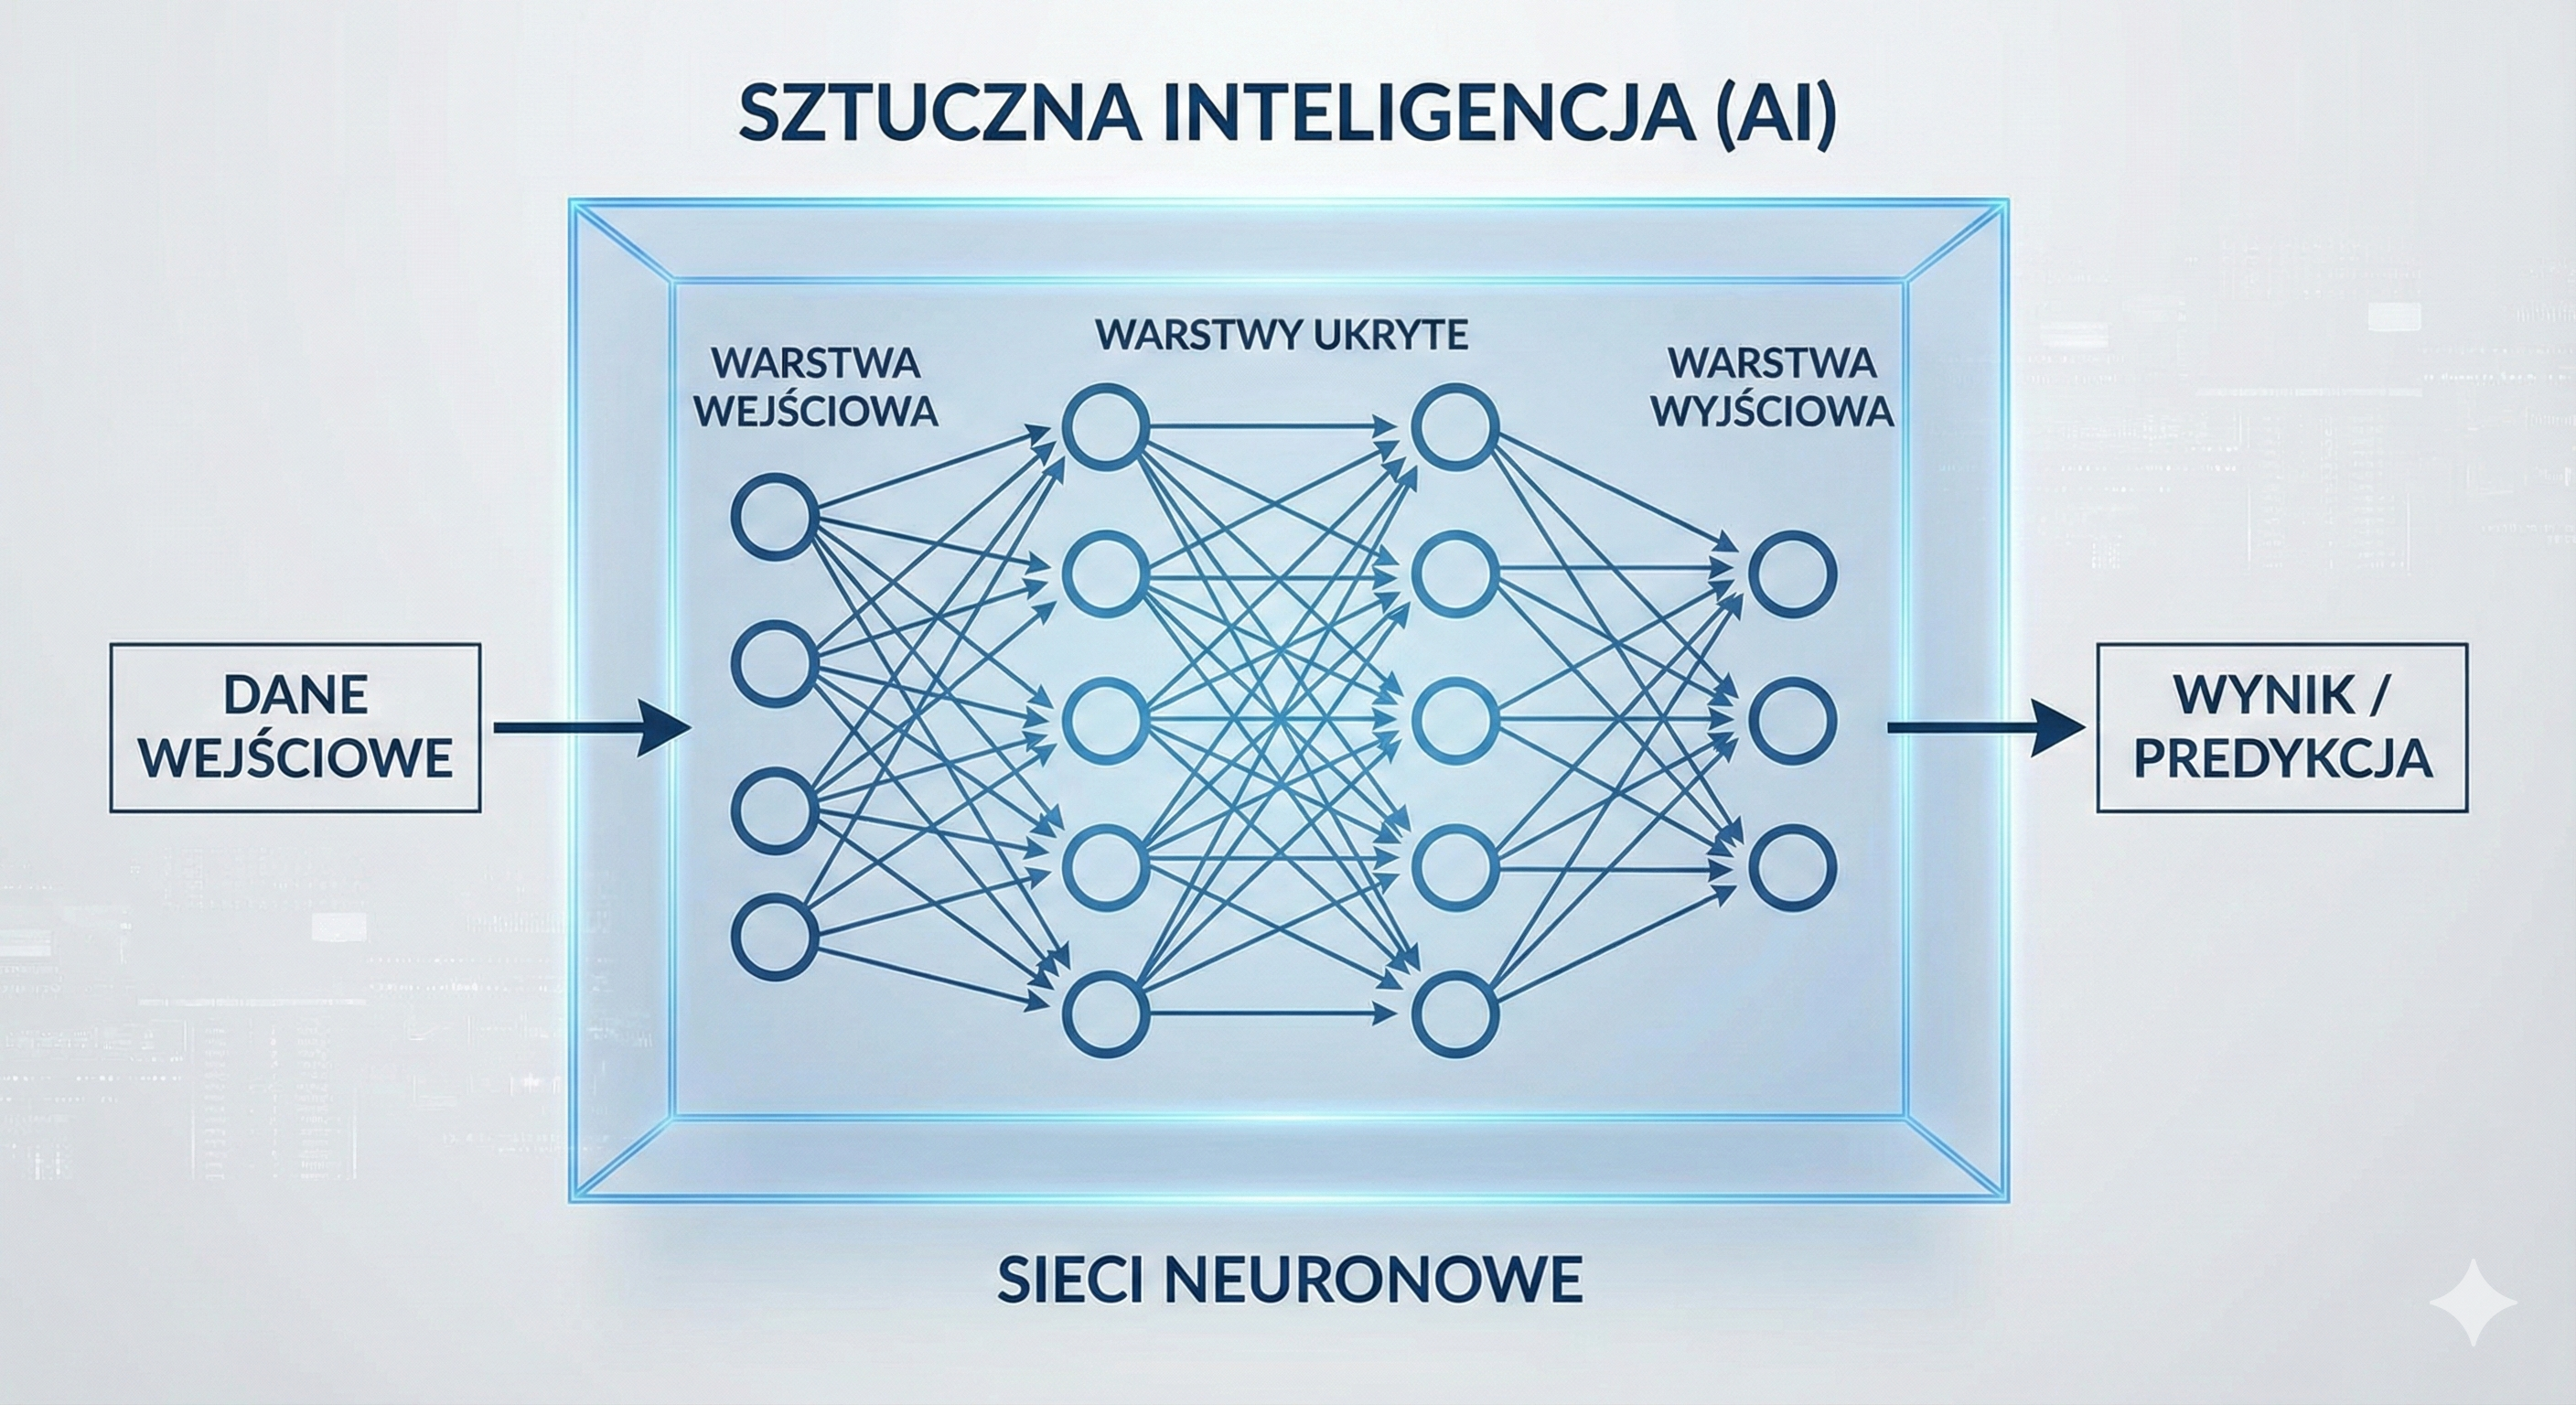
\includegraphics[width=0.9\textwidth]{obrazek.png}
    \caption{Schemat koncepcyjny sztucznej inteligencji i sieci neuronowych. Źródło: Obraz został wygenerowany za pomocą sztucznej inteligencji}
    \label{fig:siec}
\end{figure}

Jak podaje raport techniczny OpenAI, skalowanie tych modeli (zwiększanie ich rozmiaru i ilości danych) prowadzi do pojawienia się tzw. emergentnych zdolności, których nie przewidziano na etapie projektowania \cite{openai2023}. Oznacza to, że systemy te stają się coraz bardziej nieprzewidywalne, co rodzi nowe wyzwania w zakresie bezpieczeństwa AI.
\chapter{Wnioski}

\section{Podsumowanie merytoryczne}
Sztuczna inteligencja jest dynamicznie rozwijającą się dziedziną, która transformuje niemal każdy aspekt ludzkiego życia. Niniejszy dokument zaprezentował jej krótki rys historyczny, od teoretycznych rozważań Turinga po współczesne modele generatywne. Omówiono również podział na słabą (ANI) i silną (AGI) sztuczną inteligencję oraz wskazano kluczowe przykłady zastosowań praktycznych.

\section{Uzasadnienie doboru narzędzi (LaTeX)}
Do wykonania niniejszego dokumentu świadomie wybrano klasę \texttt{report}. Decyzja ta została podyktowana specyfiką zadania oraz strukturą treści. Klasa \texttt{report} jest optymalna dla prac zaliczeniowych i sprawozdań technicznych z następujących powodów:
\begin{itemize}
    \item \textbf{Struktura hierarchiczna} -- Klasa ta natywnie obsługuje podział na rozdziały (\texttt{chapter}), co pozwala na logiczne wyodrębnienie poszczególnych części tematycznych (Wstęp, Historia, Zastosowania). Jest to funkcja niedostępna w klasie \texttt{article}.
    \item \textbf{Formatowanie} -- W przeciwieństwie do klasy \texttt{book}, klasa \texttt{report} jest domyślnie jednostronna i nie wymusza skomplikowanych reguł typograficznych (np. rozpoczynania rozdziałów zawsze na nieparzystej stronie), co czyni ją idealną do generowania cyfrowych dokumentów PDF.
    \item \textbf{Automatyzacja} -- Wykorzystanie systemu \LaTeX{} pozwoliło na automatyczne wygenerowanie spisu treści, bibliografii oraz numeracji tabel i rysunków, co znacznie podnosi estetykę i czytelność pracy.
\end{itemize}

\section{Repozytorium źródeł}
Zgodnie z wymaganiami zadania, pełny kod źródłowy tego projektu został umieszczony w systemie kontroli wersji. Jest on dostępny w publicznym repozytorium pod adresem:

\begin{center}
% Link do repozytorium github
    \url{https://github.com/MikolajZdybiewski/ZadanieLaTeX}
\end{center}

% --- Bibliografia ---
\newpage
\printbibliography[heading=bibintoc, title={Bibliografia}]

\end{document}